% Created by tikzDevice version 0.12.6 on 2025-04-07 10:11:05
% !TEX encoding = UTF-8 Unicode
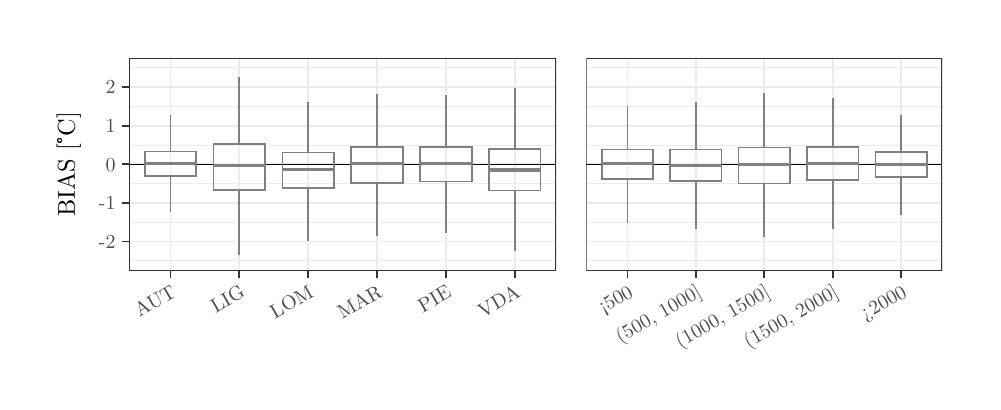
\begin{tikzpicture}[x=1pt,y=1pt]
\definecolor{fillColor}{RGB}{255,255,255}
\path[use as bounding box,fill=fillColor] (0,0) rectangle (341.43,128.04);
\begin{scope}
\path[clip] (  0.00,  0.00) rectangle (341.43,128.04);
\definecolor{drawColor}{RGB}{255,255,255}

\path[draw=drawColor,line width= 0.6pt,line join=round,line cap=round,fill=fillColor] (  0.00,  0.00) rectangle (341.43,128.04);
\end{scope}
\begin{scope}
\path[clip] (  5.50,  5.50) rectangle (196.41,122.54);
\definecolor{drawColor}{RGB}{255,255,255}
\definecolor{fillColor}{RGB}{255,255,255}

\path[draw=drawColor,line width= 0.6pt,line join=round,line cap=round,fill=fillColor] (  5.50,  5.50) rectangle (196.41,122.54);
\end{scope}
\begin{scope}
\path[clip] (196.41,  5.50) rectangle (335.93,122.54);
\definecolor{drawColor}{RGB}{255,255,255}
\definecolor{fillColor}{RGB}{255,255,255}

\path[draw=drawColor,line width= 0.6pt,line join=round,line cap=round,fill=fillColor] (196.41,  5.50) rectangle (335.93,122.54);
\end{scope}
\begin{scope}
\path[clip] ( 36.68, 40.29) rectangle (190.91,117.04);
\definecolor{fillColor}{RGB}{255,255,255}

\path[fill=fillColor] ( 36.68, 40.29) rectangle (190.91,117.04);
\definecolor{drawColor}{gray}{0.92}

\path[draw=drawColor,line width= 0.3pt,line join=round] ( 36.68, 43.78) --
	(190.91, 43.78);

\path[draw=drawColor,line width= 0.3pt,line join=round] ( 36.68, 57.73) --
	(190.91, 57.73);

\path[draw=drawColor,line width= 0.3pt,line join=round] ( 36.68, 71.69) --
	(190.91, 71.69);

\path[draw=drawColor,line width= 0.3pt,line join=round] ( 36.68, 85.64) --
	(190.91, 85.64);

\path[draw=drawColor,line width= 0.3pt,line join=round] ( 36.68, 99.59) --
	(190.91, 99.59);

\path[draw=drawColor,line width= 0.3pt,line join=round] ( 36.68,113.55) --
	(190.91,113.55);

\path[draw=drawColor,line width= 0.6pt,line join=round] ( 36.68, 50.75) --
	(190.91, 50.75);

\path[draw=drawColor,line width= 0.6pt,line join=round] ( 36.68, 64.71) --
	(190.91, 64.71);

\path[draw=drawColor,line width= 0.6pt,line join=round] ( 36.68, 78.66) --
	(190.91, 78.66);

\path[draw=drawColor,line width= 0.6pt,line join=round] ( 36.68, 92.62) --
	(190.91, 92.62);

\path[draw=drawColor,line width= 0.6pt,line join=round] ( 36.68,106.57) --
	(190.91,106.57);

\path[draw=drawColor,line width= 0.6pt,line join=round] ( 51.61, 40.29) --
	( 51.61,117.04);

\path[draw=drawColor,line width= 0.6pt,line join=round] ( 76.48, 40.29) --
	( 76.48,117.04);

\path[draw=drawColor,line width= 0.6pt,line join=round] (101.36, 40.29) --
	(101.36,117.04);

\path[draw=drawColor,line width= 0.6pt,line join=round] (126.23, 40.29) --
	(126.23,117.04);

\path[draw=drawColor,line width= 0.6pt,line join=round] (151.11, 40.29) --
	(151.11,117.04);

\path[draw=drawColor,line width= 0.6pt,line join=round] (175.98, 40.29) --
	(175.98,117.04);
\definecolor{drawColor}{RGB}{0,0,0}

\path[draw=drawColor,line width= 0.1pt,line join=round] ( 36.68, 78.66) -- (190.91, 78.66);
\definecolor{drawColor}{gray}{0.50}

\path[draw=drawColor,line width= 0.6pt,line join=round] ( 51.61, 83.33) -- ( 51.61, 96.51);

\path[draw=drawColor,line width= 0.6pt,line join=round] ( 51.61, 74.55) -- ( 51.61, 61.40);

\path[draw=drawColor,line width= 0.6pt] ( 42.28, 83.33) --
	( 42.28, 74.55) --
	( 60.94, 74.55) --
	( 60.94, 83.33) --
	( 42.28, 83.33) --
	cycle;

\path[draw=drawColor,line width= 1.1pt] ( 42.28, 78.94) -- ( 60.94, 78.94);

\path[draw=drawColor,line width= 0.6pt,line join=round] ( 76.48, 86.02) -- ( 76.48,110.31);

\path[draw=drawColor,line width= 0.6pt,line join=round] ( 76.48, 69.46) -- ( 76.48, 45.84);

\path[draw=drawColor,line width= 0.6pt] ( 67.15, 86.02) --
	( 67.15, 69.46) --
	( 85.81, 69.46) --
	( 85.81, 86.02) --
	( 67.15, 86.02) --
	cycle;

\path[draw=drawColor,line width= 1.1pt] ( 67.15, 78.26) -- ( 85.81, 78.26);

\path[draw=drawColor,line width= 0.6pt,line join=round] (101.36, 82.90) -- (101.36,101.14);

\path[draw=drawColor,line width= 0.6pt,line join=round] (101.36, 70.04) -- (101.36, 50.99);

\path[draw=drawColor,line width= 0.6pt] ( 92.03, 82.90) --
	( 92.03, 70.04) --
	(110.69, 70.04) --
	(110.69, 82.90) --
	( 92.03, 82.90) --
	cycle;

\path[draw=drawColor,line width= 1.1pt] ( 92.03, 76.76) -- (110.69, 76.76);

\path[draw=drawColor,line width= 0.6pt,line join=round] (126.23, 84.86) -- (126.23,104.07);

\path[draw=drawColor,line width= 0.6pt,line join=round] (126.23, 71.98) -- (126.23, 52.71);

\path[draw=drawColor,line width= 0.6pt] (116.91, 84.86) --
	(116.91, 71.98) --
	(135.56, 71.98) --
	(135.56, 84.86) --
	(116.91, 84.86) --
	cycle;

\path[draw=drawColor,line width= 1.1pt] (116.91, 78.89) -- (135.56, 78.89);

\path[draw=drawColor,line width= 0.6pt,line join=round] (151.11, 85.03) -- (151.11,103.74);

\path[draw=drawColor,line width= 0.6pt,line join=round] (151.11, 72.48) -- (151.11, 53.67);

\path[draw=drawColor,line width= 0.6pt] (141.78, 85.03) --
	(141.78, 72.48) --
	(160.44, 72.48) --
	(160.44, 85.03) --
	(141.78, 85.03) --
	cycle;

\path[draw=drawColor,line width= 1.1pt] (141.78, 78.87) -- (160.44, 78.87);

\path[draw=drawColor,line width= 0.6pt,line join=round] (175.98, 84.23) -- (175.98,106.40);

\path[draw=drawColor,line width= 0.6pt,line join=round] (175.98, 69.22) -- (175.98, 47.19);

\path[draw=drawColor,line width= 0.6pt] (166.66, 84.23) --
	(166.66, 69.22) --
	(185.31, 69.22) --
	(185.31, 84.23) --
	(166.66, 84.23) --
	cycle;

\path[draw=drawColor,line width= 1.1pt] (166.66, 76.61) -- (185.31, 76.61);
\definecolor{drawColor}{gray}{0.20}

\path[draw=drawColor,line width= 0.6pt,line join=round,line cap=round] ( 36.68, 40.29) rectangle (190.91,117.04);
\end{scope}
\begin{scope}
\path[clip] (  0.00,  0.00) rectangle (341.43,128.04);
\definecolor{drawColor}{gray}{0.30}

\node[text=drawColor,anchor=base east,inner sep=0pt, outer sep=0pt, scale=  0.72] at ( 31.73, 48.29) {-2};

\node[text=drawColor,anchor=base east,inner sep=0pt, outer sep=0pt, scale=  0.72] at ( 31.73, 62.25) {-1};

\node[text=drawColor,anchor=base east,inner sep=0pt, outer sep=0pt, scale=  0.72] at ( 31.73, 76.20) {0};

\node[text=drawColor,anchor=base east,inner sep=0pt, outer sep=0pt, scale=  0.72] at ( 31.73, 90.15) {1};

\node[text=drawColor,anchor=base east,inner sep=0pt, outer sep=0pt, scale=  0.72] at ( 31.73,104.11) {2};
\end{scope}
\begin{scope}
\path[clip] (  0.00,  0.00) rectangle (341.43,128.04);
\definecolor{drawColor}{gray}{0.20}

\path[draw=drawColor,line width= 0.6pt,line join=round] ( 33.93, 50.75) --
	( 36.68, 50.75);

\path[draw=drawColor,line width= 0.6pt,line join=round] ( 33.93, 64.71) --
	( 36.68, 64.71);

\path[draw=drawColor,line width= 0.6pt,line join=round] ( 33.93, 78.66) --
	( 36.68, 78.66);

\path[draw=drawColor,line width= 0.6pt,line join=round] ( 33.93, 92.62) --
	( 36.68, 92.62);

\path[draw=drawColor,line width= 0.6pt,line join=round] ( 33.93,106.57) --
	( 36.68,106.57);
\end{scope}
\begin{scope}
\path[clip] (  0.00,  0.00) rectangle (341.43,128.04);
\definecolor{drawColor}{gray}{0.20}

\path[draw=drawColor,line width= 0.6pt,line join=round] ( 51.61, 37.54) --
	( 51.61, 40.29);

\path[draw=drawColor,line width= 0.6pt,line join=round] ( 76.48, 37.54) --
	( 76.48, 40.29);

\path[draw=drawColor,line width= 0.6pt,line join=round] (101.36, 37.54) --
	(101.36, 40.29);

\path[draw=drawColor,line width= 0.6pt,line join=round] (126.23, 37.54) --
	(126.23, 40.29);

\path[draw=drawColor,line width= 0.6pt,line join=round] (151.11, 37.54) --
	(151.11, 40.29);

\path[draw=drawColor,line width= 0.6pt,line join=round] (175.98, 37.54) --
	(175.98, 40.29);
\end{scope}
\begin{scope}
\path[clip] (  0.00,  0.00) rectangle (341.43,128.04);
\definecolor{drawColor}{gray}{0.30}

\node[text=drawColor,rotate= 30.00,anchor=base east,inner sep=0pt, outer sep=0pt, scale=  0.72] at ( 54.07, 31.07) {AUT};

\node[text=drawColor,rotate= 30.00,anchor=base east,inner sep=0pt, outer sep=0pt, scale=  0.72] at ( 78.95, 31.07) {LIG};

\node[text=drawColor,rotate= 30.00,anchor=base east,inner sep=0pt, outer sep=0pt, scale=  0.72] at (103.82, 31.07) {LOM};

\node[text=drawColor,rotate= 30.00,anchor=base east,inner sep=0pt, outer sep=0pt, scale=  0.72] at (128.70, 31.07) {MAR};

\node[text=drawColor,rotate= 30.00,anchor=base east,inner sep=0pt, outer sep=0pt, scale=  0.72] at (153.57, 31.07) {PIE};

\node[text=drawColor,rotate= 30.00,anchor=base east,inner sep=0pt, outer sep=0pt, scale=  0.72] at (178.45, 31.07) {VDA};
\end{scope}
\begin{scope}
\path[clip] (  0.00,  0.00) rectangle (341.43,128.04);
\definecolor{drawColor}{RGB}{0,0,0}

\node[text=drawColor,rotate= 90.00,anchor=base,inner sep=0pt, outer sep=0pt, scale=  0.88] at ( 17.06, 78.66) {BIAS [\textdegree C]};
\end{scope}
\begin{scope}
\path[clip] (201.91, 40.29) rectangle (330.43,117.04);
\definecolor{fillColor}{RGB}{255,255,255}

\path[fill=fillColor] (201.91, 40.29) rectangle (330.43,117.04);
\definecolor{drawColor}{gray}{0.92}

\path[draw=drawColor,line width= 0.3pt,line join=round] (201.91, 43.78) --
	(330.43, 43.78);

\path[draw=drawColor,line width= 0.3pt,line join=round] (201.91, 57.73) --
	(330.43, 57.73);

\path[draw=drawColor,line width= 0.3pt,line join=round] (201.91, 71.69) --
	(330.43, 71.69);

\path[draw=drawColor,line width= 0.3pt,line join=round] (201.91, 85.64) --
	(330.43, 85.64);

\path[draw=drawColor,line width= 0.3pt,line join=round] (201.91, 99.59) --
	(330.43, 99.59);

\path[draw=drawColor,line width= 0.3pt,line join=round] (201.91,113.55) --
	(330.43,113.55);

\path[draw=drawColor,line width= 0.6pt,line join=round] (201.91, 50.75) --
	(330.43, 50.75);

\path[draw=drawColor,line width= 0.6pt,line join=round] (201.91, 64.71) --
	(330.43, 64.71);

\path[draw=drawColor,line width= 0.6pt,line join=round] (201.91, 78.66) --
	(330.43, 78.66);

\path[draw=drawColor,line width= 0.6pt,line join=round] (201.91, 92.62) --
	(330.43, 92.62);

\path[draw=drawColor,line width= 0.6pt,line join=round] (201.91,106.57) --
	(330.43,106.57);

\path[draw=drawColor,line width= 0.6pt,line join=round] (216.74, 40.29) --
	(216.74,117.04);

\path[draw=drawColor,line width= 0.6pt,line join=round] (241.46, 40.29) --
	(241.46,117.04);

\path[draw=drawColor,line width= 0.6pt,line join=round] (266.17, 40.29) --
	(266.17,117.04);

\path[draw=drawColor,line width= 0.6pt,line join=round] (290.89, 40.29) --
	(290.89,117.04);

\path[draw=drawColor,line width= 0.6pt,line join=round] (315.60, 40.29) --
	(315.60,117.04);
\definecolor{drawColor}{RGB}{0,0,0}

\path[draw=drawColor,line width= 0.1pt,line join=round] (201.91, 78.66) -- (330.43, 78.66);
\definecolor{drawColor}{gray}{0.50}

\path[draw=drawColor,line width= 0.6pt,line join=round] (216.74, 84.01) -- (216.74, 99.90);

\path[draw=drawColor,line width= 0.6pt,line join=round] (216.74, 73.40) -- (216.74, 57.49);

\path[draw=drawColor,line width= 0.6pt] (207.47, 84.01) --
	(207.47, 73.40) --
	(226.01, 73.40) --
	(226.01, 84.01) --
	(207.47, 84.01) --
	cycle;

\path[draw=drawColor,line width= 1.1pt] (207.47, 78.90) -- (226.01, 78.90);

\path[draw=drawColor,line width= 0.6pt,line join=round] (241.46, 83.99) -- (241.46,101.20);

\path[draw=drawColor,line width= 0.6pt,line join=round] (241.46, 72.52) -- (241.46, 55.39);

\path[draw=drawColor,line width= 0.6pt] (232.19, 83.99) --
	(232.19, 72.52) --
	(250.72, 72.52) --
	(250.72, 83.99) --
	(232.19, 83.99) --
	cycle;

\path[draw=drawColor,line width= 1.1pt] (232.19, 78.13) -- (250.72, 78.13);

\path[draw=drawColor,line width= 0.6pt,line join=round] (266.17, 84.74) -- (266.17,104.27);

\path[draw=drawColor,line width= 0.6pt,line join=round] (266.17, 71.72) -- (266.17, 52.27);

\path[draw=drawColor,line width= 0.6pt] (256.90, 84.74) --
	(256.90, 71.72) --
	(275.44, 71.72) --
	(275.44, 84.74) --
	(256.90, 84.74) --
	cycle;

\path[draw=drawColor,line width= 1.1pt] (256.90, 78.45) -- (275.44, 78.45);

\path[draw=drawColor,line width= 0.6pt,line join=round] (290.89, 84.92) -- (290.89,102.65);

\path[draw=drawColor,line width= 0.6pt,line join=round] (290.89, 72.99) -- (290.89, 55.20);

\path[draw=drawColor,line width= 0.6pt] (281.62, 84.92) --
	(281.62, 72.99) --
	(300.16, 72.99) --
	(300.16, 84.92) --
	(281.62, 84.92) --
	cycle;

\path[draw=drawColor,line width= 1.1pt] (281.62, 78.85) -- (300.16, 78.85);

\path[draw=drawColor,line width= 0.6pt,line join=round] (315.60, 83.17) -- (315.60, 96.66);

\path[draw=drawColor,line width= 0.6pt,line join=round] (315.60, 74.08) -- (315.60, 60.47);

\path[draw=drawColor,line width= 0.6pt] (306.33, 83.17) --
	(306.33, 74.08) --
	(324.87, 74.08) --
	(324.87, 83.17) --
	(306.33, 83.17) --
	cycle;

\path[draw=drawColor,line width= 1.1pt] (306.33, 78.54) -- (324.87, 78.54);
\definecolor{drawColor}{gray}{0.20}

\path[draw=drawColor,line width= 0.6pt,line join=round,line cap=round] (201.91, 40.29) rectangle (330.43,117.04);
\end{scope}
\begin{scope}
\path[clip] (  0.00,  0.00) rectangle (341.43,128.04);
\definecolor{drawColor}{gray}{0.20}

\path[draw=drawColor,line width= 0.6pt,line join=round] (216.74, 37.54) --
	(216.74, 40.29);

\path[draw=drawColor,line width= 0.6pt,line join=round] (241.46, 37.54) --
	(241.46, 40.29);

\path[draw=drawColor,line width= 0.6pt,line join=round] (266.17, 37.54) --
	(266.17, 40.29);

\path[draw=drawColor,line width= 0.6pt,line join=round] (290.89, 37.54) --
	(290.89, 40.29);

\path[draw=drawColor,line width= 0.6pt,line join=round] (315.60, 37.54) --
	(315.60, 40.29);
\end{scope}
\begin{scope}
\path[clip] (  0.00,  0.00) rectangle (341.43,128.04);
\definecolor{drawColor}{gray}{0.30}

\node[text=drawColor,rotate= 30.00,anchor=base east,inner sep=0pt, outer sep=0pt, scale=  0.72] at (219.20, 31.07) {<500};

\node[text=drawColor,rotate= 30.00,anchor=base east,inner sep=0pt, outer sep=0pt, scale=  0.72] at (243.92, 31.07) {(500, 1000]};

\node[text=drawColor,rotate= 30.00,anchor=base east,inner sep=0pt, outer sep=0pt, scale=  0.72] at (268.63, 31.07) {(1000, 1500]};

\node[text=drawColor,rotate= 30.00,anchor=base east,inner sep=0pt, outer sep=0pt, scale=  0.72] at (293.35, 31.07) {(1500, 2000]};

\node[text=drawColor,rotate= 30.00,anchor=base east,inner sep=0pt, outer sep=0pt, scale=  0.72] at (318.07, 31.07) {>2000};
\end{scope}
\end{tikzpicture}
